\chapter{Representation Learning}

\section{Introduction}
% Authors: 
% Lecture date: 4/22/2019
% Slides 1 - 6

Researches have always been interested in learning about relations and interaction of components of networks and the motivation for it is what lots of science and knowledge is about. Like social science is about understanding how each component of the economy/society interact with each other i.e. Similarly in AI, researchers are interested in similar things. 

We can model these multi-relational data (relational knowledge) using entities + relationship model and use the model to do link prediction, entity resolution and community detection. 
\begin{figure}[htb!]
\centering
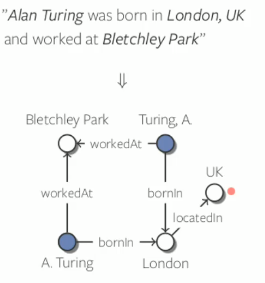
\includegraphics[width=0.5\linewidth]{lectures/11-a/slides2.PNG}
\label{fig:tag_overlap}
\caption{Entities + relationship model}
\end{figure}
i.e Given the above graph, we can predict the link that Turning is also a citizen of UK which is not given by the data.

Researchers have been trying to build very large knowledge graph and they have been successful. Examples of them includes Google knowledge graph that contain 570 million nodes and over 18 billion edges. However, there are still problems with them like data still very noisy and incomplete despite the huge size.

One naïve but decently successful way to model knowledge graph is Markov Logic Model whose main idea is to combine graphical models with probability inference. We can give probability inference based on rules given. However, there are two major problems for this model: scalability and requirement of prior knowledge.

% Slides 6 -  (for reference)
Slides 6-7:
The main idea of embedding model is to extract feature representation to explain relationship and is the formula inspired by NLP embedding i.e we can add embedding of man and women to get close to man.
However, there is problem wrt the formula (TransE) which is the symmetric relationship
F(s,p,o) != f(o,p,s)

Slides 8-9:
The way to fix the problem is to use dot product (RESCAL)
It’s equivalent to factorize a large adjacency matrix to two matrix of relationships
We explained relationship via interactions of latent features

Slides 10:
This model is good that it has decoupling effect. It gives the property that makes the model scalable.
The model is differentiable and can use gradient optimization 
Need minimal prior knowledge, only need some observation and scoring function.

Slides 11:
Task: learn to find out test countries belong to which region.
We know train belong to sub belongs to region.
Can apply to much larger and complex problems

Slides 12:
However, in the example, it seems we haven’t reached saturated point, but increasing dimensionality would make computation too hard.

Slides 13:
Lots of knowledge have underlying hierarchical structure 

Slides of 14:
Example of the tree like structure
Number of nodes grow exponentially with depth
Volume of embedding space will need to grow very fast

%%%%%%%%%%%%%%%%%%%%%
%% Begin Sreyas' part

%% Kevin writes until 37 minutes in the video. Assumes that Kevin has written the equations for score function and probabilistic mdoel. 

%%start time 36 minutes
\subsection{TransE}
TransE introduced by Bordes et al. 2013 uses a score function of the form $$ f(s, p, o) = -|| e_s + r_p - e_o ||_p $$ where $e_i$ are entity and $r_i$ are relational embedding. Note that is is basically saying that if you take the embedding of $o$ and add the embedding of relationship, you should be close to the embedding of $p$ - this is very similar to what we see in word2vec. 

This score function is particularly nice in the sense that this is very fast to compute, the running time is $\mathcal{O}(d_e)$ where $d_e$ is the embedding dimension. A particularly stricking problem with the cost function is it's inability to model symmetric relations. A relation $p$ of the form $f(s, p, o) = f(o, p, s)$ for all $s, p$ is called a symmetric relation. Note that, if $f(s, p, o) = f(o, p, s)$ is satisfied, then this implies that $r_p$ should be zero vector. Therefore, one can model only one symmetric relation using this formalism. 

\subsection{RESCAL}
RESCAL introduced by Nickel et al, 2011 uses a cost function of the form:
$$ f(s, p, o) = e_s^TRpe_o$$
Note that, unlike TransE, relational embeddings have a different size from entity embedding and we see it as a matrix. This score function takes $\mathcal{O}(d_e^2)$ making it's evaluation difficult in large graphs. 

One could think about the components of entity embedding as latent features of the entities. Note that 
$$  f(s, p, o) = e_s^TRpe_o = r_p^T(e_s \mathop{\otimes} e_o) $$ where $(e_s \mathop{\otimes} e_o)$ represents the outer product of $e_s$ and $e_o$. $(e_s \mathop{\otimes} e_o)$ may be thought of as representing a feature vector for the pair $(e_s, e_o)$ and then applying it to a linear classified with weight $r_p$ gives as the score $f(s, p, o)$

\subsection{Discussion on Relational Learning with Embedding}
\begin{figure}[htb!]
\centering
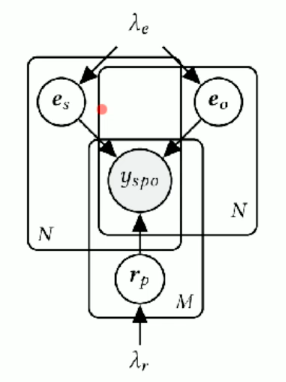
\includegraphics[width=0.5\linewidth]{lectures/11-a/relational_learning_graphical_model.png}
\label{fig:relational_learning_gm}
\caption{Graphical Model Representing Relational Learning with Embedding}
\end{figure}

Figure \ref{fig:relational_learning_gm} shows the graphical model capturing dependencies of relational learning with embedding. Some of the merits of this method are:
\begin{enumerate}
    \item \textbf{Decoupling} Unlike Markov Logic Networks, one can using do inference by doing a local computation $f(s, p, o)$
    \item \textbf{Gradient Based Optimization} The loss function is differential and the score functions $f(s, p, o)$ are also typically differentiable, which means one can use gradient based methods for learning helping to scale up easily to large datasets.
    \item \textbf{Minimal Prior Knowledge} Unlike Markov Logic Network, one need not have any prior knowledge about the problem - one can easily learn them in this framework. 
    \item \textbf{Black Box Model} Less interpretable than MLN.
\end{enumerate}


%% Ended at 01:00:00 
%% Have to write from Poincare Embedding or Hierarchical Structures and Representation Learning

%% End of Sreyas' part
%%%%%%%%%%%%%%%%%%%%%%%%%%


\section{Hierarchical representation in Hyperbolic Space}
Representation learning has become an invaluable approach for learning from symbolic data such as text and graphs. However, while complex symbolic datasets often exhibit a latent hierarchical structure, state-of-the-art methods typically learn embeddings in Euclidean vector spaces, which do not account for this property.

For example, in a tree-like graph structure, we aim to embed nodes such that the distance between the nodes is less than a given distance ‘r’ if they are connected and greater than ‘r’ otherwise.

\begin{figure}[htb!]
\centering
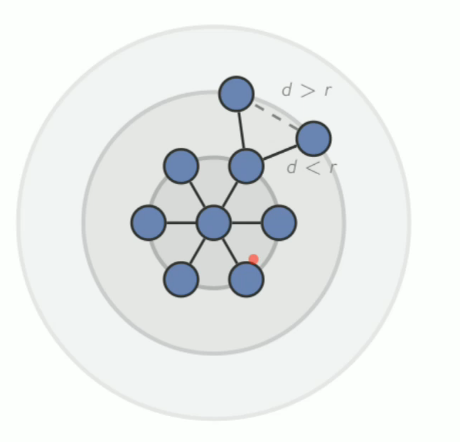
\includegraphics[width=0.5\linewidth]{lectures/11-a/tree_graphs.PNG}
\label{fig:treegraphs}
\caption{Tree-like graphs with embedded nodes having distance less than 'r' if connected and greater than 'r' otherwise}
\end{figure}

But the problem with the tree-like structure is the number of nodes grows exponentially with depth. Thus, as the radius of the graph increases, to maintain the above-mentioned rule for distance, the volume needs to also grow exponentially. This exponential growth of volume is not possible in Euclidean space thus the only possible way to address this need for exponential growth is through increasing the dimensionality. The limitations with increasing the dimensionality are 1) its expensive in terms of memory for computation 2) it only conserves topology/structure rather than semantics, which is of actual importance for our model learning.
\begin{figure}
\centering
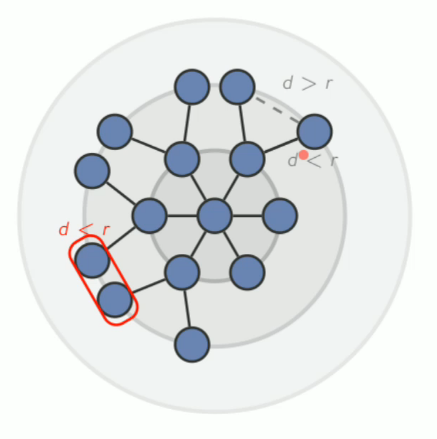
\includegraphics[width=0.5\linewidth]{lectures/11-a/tree_graphs_limitation.PNG}
\caption{Limitation of representation of tree-like graphs in Euclidean Space when the depth increases.}
\end{figure}


A better way for geometric representation of a tree-based graph is by calculating the similarity in hyperbolic space rather than the Euclidean space. The geometrical properties which make hyperbolic space more suitable for this task are 1) It is a continuous analog of trees 2) It acts as geometric prior for hierarchies 3) it is still a Riemann manifold which enables the use of gradient-based optimization to compute embeddings.

\subsection{Poincaré Embeddings for
Learning Hierarchical Representations}

The most intuitive example of hyperbolic space for representation learning is the Poincare Ball Model. Poincare Ball Model is a new approach for learning hierarchical representations of symbolic data by embedding them into hyperbolic space – or more precisely into an n-dimensional Poincaré ball. Due to the underlying hyperbolic geometry, this allows learning parsimonious representations of symbolic data by simultaneously capturing hierarchy and similarity.

\begin{figure}[htb!]
\centering
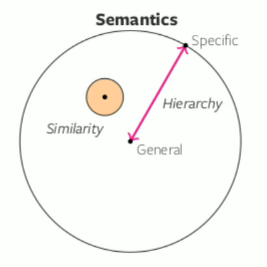
\includegraphics[width=0.5\linewidth]{lectures/11-a/poincareball_semantics.PNG}
\label{fig:relational_learning_gm}
\caption{Modelling Semantics in Poincare Ball Model}

\end{figure}

For modeling tree-like structure in the Poincare ball 1) the roots are points at the origin which are relatively close to all points 2) leaves are points at the boundary which are far apart from most of the points 3) the shortest paths are the geodesics which go through more general points.

\begin{figure}[htb!]
\centering
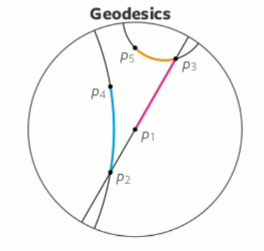
\includegraphics[width=0.5\linewidth]{lectures/11-a/poincareball_geodesics.PNG}
\label{fig:relational_learning_gm}
\caption{Geodesics in Poincare Ball Models}
\end{figure}

